\documentclass{beamer}

\usepackage[francais]{babel}
\usepackage[T1]{fontenc}
\usepackage[utf8]{inputenc}
\usepackage{beamerthemecs}
\usepackage{beamerouterthemecs}
\usepackage{beamerfontthemecs}
\usepackage{beamerinnerthemecs}
\usepackage{beamercolorthemecs}

\usetheme{cs}
\useoutertheme{cs}
\usefonttheme{cs}
\useinnertheme{cs}
\usecolortheme{cs}

\title[Visualisation de traces réseaux]{Visualisation de traces réseaux}
\author{\textbf{Thibault \textsc{Lengagne}et Nicolas \textsc{Ngô-Maï}}}
\institute{Centrale Supélec - Campus de Rennes}

\begin{document}

  \begin{frame}
    \titlepage
  \end{frame}
  
  \AtBeginSection[] {
    \begin{frame}
      \frametitle{Plan}
      \tableofcontents[currentsection, hideothersubsections, pausesubsections]
    \end{frame} 
  }

 \section{Retour sur les choix technologiques}
  \begin{frame}
    \frametitle{Rappel du Sujet}
    \begin{itemize}
     \item Le but est de créer un outil destiné aux pentesters, permettant d'analyser efficacement une trace réseau.
     \item L'attaquant dispose d'une trace réseau mais n'a aucune connaissance de ce réseau.
     \item Un fichier pcap devient rapidement très volumineux et son analyse est laborieuse, nécessitant l'utilisation de plusieurs outils.
    \end{itemize}
  \end{frame}
  
  \begin{frame}
    \frametitle{Rappel du Sujet}
    L'attaquant espère soutirer des informations sur le réseau :
    \begin{itemize}
      \item Les adresse IP identifiées ( + géolocalisation, résolution DNS)
      \item Les protocoles utilisés ( en particulier non chiffrés ou mal configurés)
      \item Les noeuds importants du réseau (serveur de fichier, DNS, LDAP...)
      \item Extraire des traces réseaux filtrées, extraire les données sensibles
    \end{itemize}
  \end{frame}

  \begin{frame}
   \frametitle{Retour sur les choix technologiques}
    \begin{itemize}
      \item Nous voulions à l'origine interfacer plusieurs outils (Ettercap, ChaosReader, tcptrace...) 
      \item Finalement, Scapy nous permet de manipuler la trace réseau de façon satisfaisante.
      \item Enfin, le choix initial de PyQt a été remplacé par une interface web.
    \end{itemize}
  \end{frame}
  
  \begin{frame}
  \frametitle{Resumé des choix technologiques}
   \begin{itemize}
    \item Pour stocker les résultats, nous avons choisi d'utiliser une base de donnée PostGreSQL
    \item Nous avons trouvé un outil très puissant pour faire de la visualisation : D3.js
    \item Nous avons donc choisi de mettre en place un serveur web en python (Flask)
   \end{itemize}
  \end{frame}
  
  \begin{frame}
  \frametitle{Retour sur les objectifs fixés}
    Nous avons d'ores et déjà remplis les objectifs suivants :
    \begin{itemize}
     \item Extraction de sessions, des utilisateurs, et des protocoles
     \item Création de statistiques, extraction des données en clair
     \item Visualisation en barre parallèle
    \end{itemize}
  \end{frame}
  
  \section{Détails techniques}
  \begin{frame}
   Quatres tables dans la base de données :
   \begin{center}
    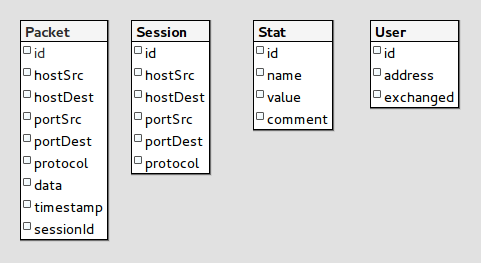
\includegraphics[scale=0.6]{postgre.png}
   \end{center}
  \end{frame}
  
  \begin{frame}
    \frametitle{Analyse du fichier pcap}
    \begin{itemize}
     \item La libraire Scapy permet de lire nos fichiers, puis de manipuler les packets.
     \item Une fonction parcourt tous les paquets. Les tables User et Stats sont alimentées 
     \item Une fonction parcourt tous les sessions. Les tables Session et Trames sont alimentées
    \end{itemize}
    %Montrer le code réduit
  \end{frame}
  
  \begin{frame}
    \frametitle{Performances du parser}
    \begin{itemize}
     \item Les fichiers pcap peuvent atteindre plusieurs Giga assez rapidement. 
     \item L'écriture dans la base de donnée étant couteuse,le programme écrit dans la base de donnée une seule fois, à la fin de la collecte des données
    \end{itemize}
    %Afficher les résultats
  \end{frame}
  
  \begin{frame}
    \begin{center}
      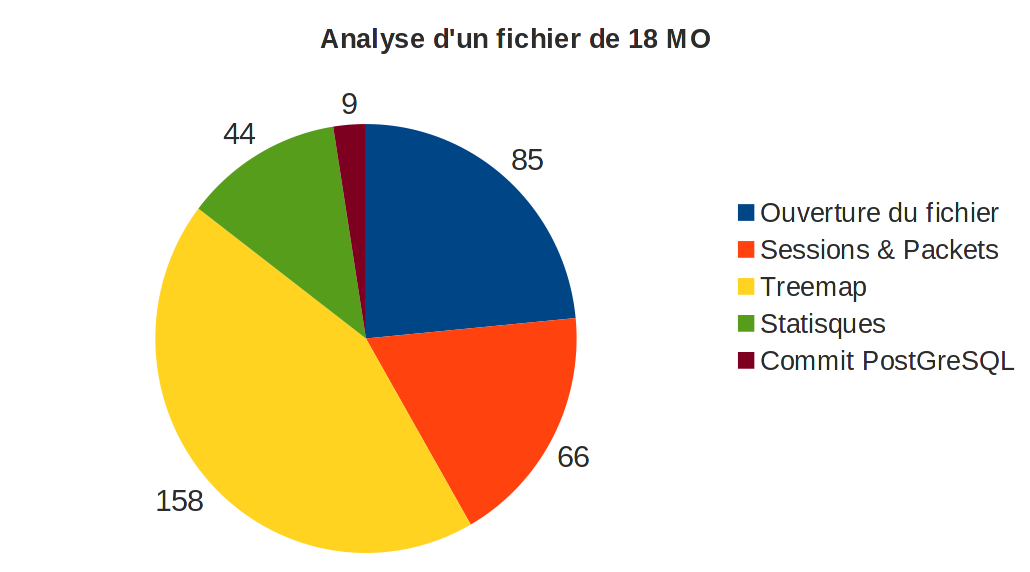
\includegraphics[scale=0.3]{parse-time.png}
    \end{center} 
  \end{frame}
  
  \begin{frame}
    \begin{center}
       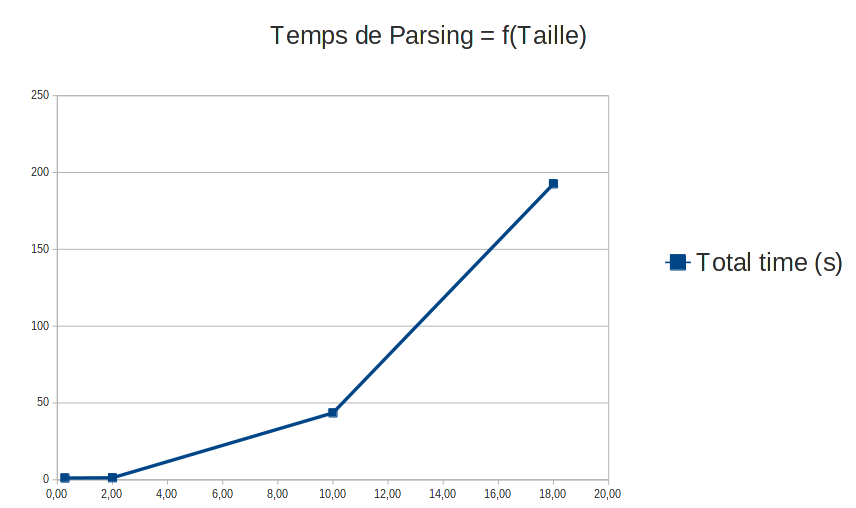
\includegraphics[scale=0.3]{parse-temps.png}
    \end{center} 
  \end{frame}

  
 \section{Démonstration}
  \begin{frame}
    \frametitle{Lancement de l'outil}
    Le projet est disponible sur https://github.com/lechinoix/Pcap-visualization-project \\
    Après avoir suivi la procédure d'installation, on démarre le serveur pour accéder à l'interface web \\
  \end{frame}

  %Ici une démonstration live de 5 min

  \section{Travail à venir}
  \begin{frame}
    Objectifs à remplir
    \begin{itemize}
     \item Ajouter les différents filtres possibles
     \item Extraire d'un pcap a partir des trames filtrées
     \item Extraire les données non chiffrées des protocoles SMTP,IMAP,POP,LDAP
     \item Ajouter la résolution DNS
     \item Ajouter d'autres mode de visualisation (carte des IP,..)
    \end{itemize}
  \end{frame}


  \section{Conclusion}
  \begin{frame}
    \begin{center}
      Merci de votre attention !
    \end{center}
  \end{frame}

\end{document}
